%tag:000Y
%label:art:viterbosTheorem
%author:JeffHicks
%name:"Viterbo's theorem"
%type:article

    One of the most striking computations for symplectic cohomology comes from Viterbo's theorem, which relates the symplectic cohomology of $T^*Q$ with the homology of the free loop space $\mathcal L Q$.
    %label:"def:DGModule"
%author:JeffHicks
%name:"free loop space"
%type:"definition"

 
    Let $Q$ be a manifold. The free loop space of $Q$, denote by $\mathcal L Q$, consists of all continuous maps 
    \[\gamma:S^1\to Q.\]
    The projection to base point is the map 
    \begin{align*}
        \ev_0: \mathcal L Q\to& Q\\
        \gamma\mapsto &\gamma(0).
    \end{align*}
    \label{def:freeLoopSpace}
 
    We usually regard the Hamiltonian Floer cohomology of $X$ as being ``inspired'' by doing Morse theory on the free loop space of $\Omega X$. However, it is \emph{not} the Morse theory on the loop space, which can actually be done!

    From the data of $g$ a metric for $Q$, we can define an energy functional on the space of loops of Sobelov class $W^{1,2}$,
    \begin{align*}
        E: \mathcal LQ\to \RR\\
        \gamma\mapsto \int_{\gamma}|\gamma'|^2_gdt,
    \end{align*}
    whose critical points are either constant loops or $g$-geodesics on $Q$. 
    This functional is only Morse-Bott for generic metrics (observe that every geodesic can be reparameterized) but still satisfies the property that the critical submanifolds have finite index. Therefore, the downward flow spaces of each critical submanifold is a finite dimensional submanifold, and the union of all such manifolds recovers the homotopy type of $\mathcal LQ$. Additionally, there is an honest gradient flow of $E$ --- that is, from a given loop $\gamma$ we can construct a unique $E$-gradient flow-line starting at $\gamma$. Since the gradient of $E$ points inwards along its level sets,  $CM_\bullet(\mathcal LQ, E)$ computes the \emph{homology} of the loop space.

    Given $(X, \omega, J)$ a symplectic manifold, the Floer action functional \cref{eqn:floerAction} does not have critical points of finite index or co-index --- so there are no well defined downward flow spaces, and no absolute index. Even worse, the gradient ``flow'' of the Floer action functional is not well defined (in that we don't have unique 1-dimensional families of solutions given an intial starting parameter). However, the space of gradient flow-lines between two critical points is still well-behaved, which is enough to get a ``Morse-like'' cohomology theory from $A_{H_t}:\mathcal L X \to \RR$.

    Despite these apparent differences, there is a scenario where we can translate Floer theory to study the homology of the loop space. Let $(Q, g)$ be a Riemannian manifold. Let $B^*Q$ be the unit cotangent ball. This is a Liouville domain (depending on the choice of metric $g$), whose contact boundary $(S^*Q, \alpha)$ has Reeb orbits corresponding to the $g$-geodesics of $Q$ (\cref{exr:geodesicsInSymplecticCohomology}). So, it seems reasonable to  conjecture a relation between 
    \[\text{Floer functional $A_{H}:\mathcal L(T^*Q)\to \RR$}\Leftrightarrow\text{Energy functional $E:\mathcal Q\to \RR$}\]

    We also have the suggestive relations between cohomology theories which we know how to compute:
    %tag:000X
%label:"dig:viterboSuggestive"
%type:"diagram"
%author:JeffHicks

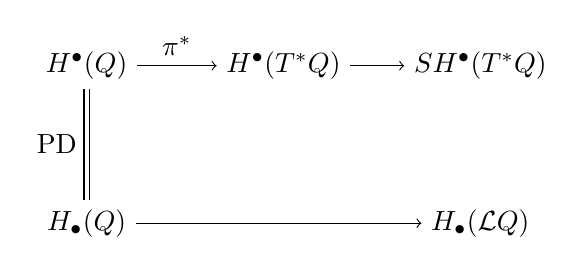
\begin{tikzpicture}

\node (v3) at (-2.5,1.5) {$H^\bullet(Q)$};
\node (v4) at (-2.5,-0.5) {$H_\bullet(Q)$};
\node (v1) at (0,1.5) {$H^\bullet(T^*Q)$};
\node (v5) at (2.5,-0.5) {$H_\bullet(\mathcal L Q)$};
\node (v2) at (2.5,1.5) {$SH^\bullet(T^*Q)$};

\draw  (v1) edge[->]  (v2);
\draw  (v3) edge[->]node[above]{$\pi^*$} (v1);
\draw  (v4) edge[->] (v5);
\draw  (v3) edge[double equal sign distance] node[left]{PD} (v4);
\end{tikzpicture}
    where the bottom arrow is inclusion of $Q\into \mathcal LQ$ by the constant loops, and the top right arrow is given by \cref{prp:homologyIncludesIntoSH}. From these pieces of evidence one might expect the following theorem. 

    %tag:000Y
%label:"thm:viterbosTheorem"
%author:JeffHicks
%name:"Viterbo's theorem"
%type:"theorem"
%source:viterbo1999functors

    Let $(Q, g)$ be a compact Riemannian manifold. Let $X=B^*Q$ be the unit cotangent ball. Then 
    \[\SH(X)= H_\bullet(\mathcal L Q).\]
    \label{thm:viterbosTheorem}


    %tag:000T
%label:"app:viterboVanishing"
%author:JeffHicks
%name:"exact Lagrangians contribute to symplectic cohomology"
%type:"application"
%parent:thm:viterbosTheorem

\begin{application}
 \label{app:viterboVanishing}
    We now look at an application of Viterbo's theorem.
    Let $X$ be a Liouville domain, and suppose that there exists $L\subset X$ an exact Lagrangian submanifold. Then a Weinstein neighborhood $B^*L\subset X$ provides an example of a Liouville subdomain. We therefore have a unital ring homomorphism $\SH(X)\to \SH(B^*L)$. Since the latter is isomorphic (as a vector space) to $H_\bullet(\mathcal L)$, it is non-vanishing. Since a unital ring homomorphism to a non-trivial target cannot have trivial domain, we conclude that $\SH(X)$ is non-vanishing.

    This application is more striking in the reverse direction. Let $X$ be a Liouville domain with vanishing symplectic cohomology (for instance, a subcritical Stein domain). Then $X$ contains no exact Lagrangian submanifolds.   
\end{application}

